\section{Kristallstruktur}

Kristalle zeichnen sich dadurch aus, dass sie im Raum periodisch sind. Man beschreibt sie durch ein Raumgitter und eine Basis. Ein Gittervektor hat die Form
\begin{equation}
 \vec{R} = \sum_{1}^{3} n_{i}\vec{a}_{i}, \qquad n_{i}\in \mathbb{Z},
\end{equation}
wobei die $\vec{a}_{i}$ die primitive Einheitszelle des Raumgitters aufspannen.

Man definiert das reziproke Gitter durch die primitiven Einheitsvektoren
\begin{equation}
 \vec{A}_{1} = \frac{2\pi}{V} \vec{a}_{2}\times\vec{a}_{3},
\end{equation}
und zyklisch, wobei $V=\vec{a}_{1}\cdot\left(\vec{a}_{2}\times\vec{a}_{3}\right)$ das Volumen der primitiven Einheitszelle des Raumgitters ist. Die $1.$ Brillouin-Zone wird definiert als die Wigner-Seitz-Zelle des reziproken Gitters. Die Wigner-Seitz-Zelle ist eine besondere primitive Einheitszelle, die sich für jedes Gitter eindeutig konstruieren lässt.

In einem eindimensionalen Gitter mit Gitterkonstante $a$ ist die $1.$ Brillouin-Zone gerade das Intervall $-\frac{\pi}{a}\leq k \leq \frac{\pi}{a}$.

\section{Gitterschwingungen: eindimensionales Modell}

In einem Kristall können die Atome zu gekoppelten Schwingungen um ihre Gleichgewichtslage angeregt werden. Die Quanten dieser Schwingungen heißen Phononen. Zur Beschreibung der Schwingungen kann ein eindimensionales Modell mit folgenden Näherungen verwendet werden:
\begin{itemize}
  \item Nächste-Nachbarn-Näherung: Es wird angenommen, dass ein Atom jeweils nur mit den nächsten Nachbarn wechselwirkt, da das Paarpotential zum übernächsten Atom sehr weit abgefallen ist.
  \item Punktmassennäherung: Die Atome werden durch Punktmassen genähert.
  \item Harmonische Näherung: Es werden kleine Auslenkungen der Atome aus ihrer Gleichgewichtslage $x_{0}$ angenommen. Dann kann das Paarpotential in eine Taylorreihe entwickelt werden:
      \begin{equation}
       V(x) \approx V(x_{0}) +\frac{1}{2} \frac{\d^{2}V}{\d x^{2}}\rvert_{x=x_{0}} \left(x-x_{0}\right)^{2}, 
      \end{equation}
      Dieses Potential kann also durch Federn mit linearer Rückstellkraft simuliert werden. Es gilt dann für die Federkonstante $D$
      \begin{equation}
       D = \frac{\d^{2}V}{\d x^{2}}|_{x=x_{0}}.
      \end{equation}
\end{itemize}
Insgesamt werden die Gitterschwingungen also durch die Schwingungen von mit Federn gekoppelten Punktmassen beschrieben.

\section{Einatomige Kette}

Betrachte nun Punktmassen der Masse $m$, die mit Federn mit Federkonstante $D$ verbunden sind (s. Abb. \ref{fig:1d_kette}). Der Gleichgewichtsabstand sei $a$. Die Auslenkung der $j$-ten Punktmasse sei $s_{j}$. Die Bewegungsgleichung für $s_{j}$ lautet dann
\begin{equation}
  m\ddot{s}_{j} = D\left( s_{j+1} + s_{j-1} -2s_{j} \right).
\end{equation}
Der Ansatz
\begin{equation}
 s_{j}(t) = A \e^{i(kaj-\omega t)},
\end{equation}
führt auf die Dispersionsrelation
\begin{equation}
 \omega(k) = \sqrt{\frac{4D}{m}} \left|\sin\left(\frac{ka}{2}\right)\right|.
\end{equation}
Es ist zu erkennen, dass die Dispersionsrelation periodisch von $k$ abhängt, mit der Periode $\frac{2\pi}{a}$ (graphische Darstellung: Abb. \ref{fig:brillouin_1}). Dies entspricht gerade der Länge der $1.$ Brillouin-Zone. Es genügt also Wellenzahlen in der ersten Brillouin-Zone zu betrachten. Der physikalische Grund dafür ist, dass die Auslenkung der Welle nur an einigen diskreten Punkten betrachtet wird. Ändert man den Wellenvektor um einen reziproken Gittervektor, so verändert sich die Auslenkung an diesen Punkten nicht. Wellen bei denen $\vec{k}$ um einen reziproken Gittervektor verschoben ist, sind also physikalisch nicht unterscheidbar (s. Abb. \ref{fig:auslenkung}).

\begin{figure}[tb]
  \centering
  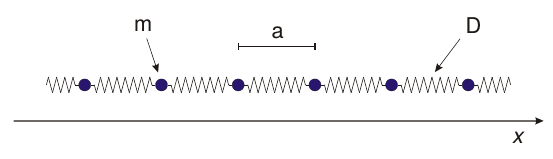
\includegraphics[scale=1.0]{./fig/1d_kette.png}
  \caption{Schematische Darstellung einer eindimensionalen Kette aus mit Federn gekoppelten Punktmassen \cite{Litmap}}
  \label{fig:1d_kette}
\end{figure}

\begin{figure}[tb]
  \centering
  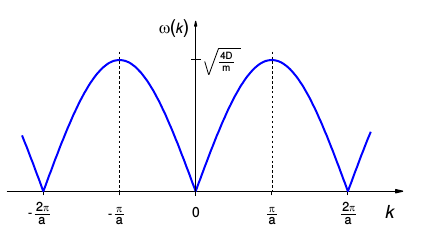
\includegraphics[scale=1.0]{./fig/brillouin_1.png}
  \caption{Dispersionsrelation der eindimensionalen Kette \cite{Litmap}}
  \label{fig:brillouin_1}
\end{figure}

\begin{figure}[tb]
  \centering
  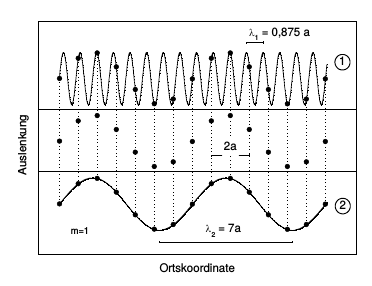
\includegraphics[scale=1.0]{./fig/auslenkung.png}
  \caption{Schematische Darstellung von Wellen, deren Wellenzahl um einen reziproken Gittervektor verschoben ist. Es ist zu erkennen, dass sich die Auslenkung an den Gitterpunkten nicht unterscheidet. \cite{Litmap}}
  \label{fig:auslenkung}
\end{figure}

\subsection{Diskussion der Lösung}

Die Phasengeschwindigkeit einer Welle ist definiert als
\begin{equation}
 v_{ph} = \frac{\omega}{k},
\end{equation}
und die Gruppengeschwindigkeit als
\begin{equation}
 v_{gr} = \pdb{\omega}{k}.
\end{equation}
Im Zentrum der Brillouin-Zone kann die Dispersionsrelation linear genähert werden
\begin{equation}
 \omega(k) \approx \sqrt{\frac{4D}{m}} \frac{a}{2} \lvert k\rvert .
\end{equation}
Somit ergibt sich
\begin{equation}
 v_{ph} = v_{gr} = a\sqrt{\frac{D}{m}}.
\end{equation}
Dies ist gerade die Schallgeschwindigkeit im Medium. Schon bei sehr niedrigen Anregungsenergien kommt es zum Transport von Schallwellen mit dieser Geschwindigkeit.

Am Rand der ersten Brillouin-Zone gilt
\begin{equation}
 v_{gr} = \pdb{\omega}{k} = 0.
\end{equation}
Es handelt sich also um Wellen, die sich nicht ausbreiten, sogenannte stehende Wellen. Deren Auftreten lässt sich folgendermaßen verstehen: eine einlaufende Welle mit $k=\frac{\pi}{a}$ wird im Kristall Bragg-reflektiert zu einer Welle mit $k=-\frac{\pi}{a}$.
Dabei handelt es sich um eine Welle mit der gleichen Wellenlänge, die sich in entgegengesetzter Richtung ausbreitet. Die beiden Wellen interferieren und es entsteht eine stehende Welle. 

\section{Zweiatomige Kette}

Nun wird eine lineare Kette aus zwei Punktmassen unterschiedlicher Masse ($m$ und $M$) betrachtet. Die Massen sind jeweils abwechselnd im Abstand $\frac{a}{2}$ angeordnet (s. Abb. \ref{fig:2d_kette}). Dies ist ein Modell für einen Kristall mit Gitterkonstante $a$ und einer zweiatomigen Basis.

\begin{figure}[tb]
  \centering
  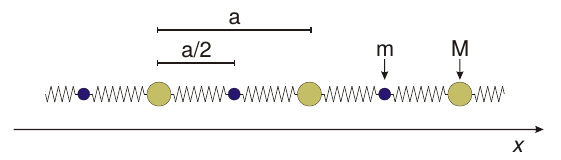
\includegraphics[scale=1.0]{./fig/2d_kette.png}
  \caption{Schematische Darstellung einer eindimensionalen zweiatomigen Kette aus mit Federn gekoppelten Punktmassen \cite{Litmap}}
  \label{fig:2d_kette}
\end{figure}

\begin{figure}[tb]
  \centering
  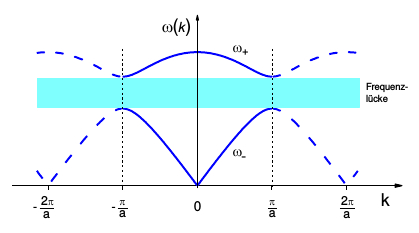
\includegraphics[scale=1.0]{./fig/brillouin_2.png}
  \caption{Dispersionsrelation der zweiatomigen Kette \cite{Litmap}}
  \label{fig:brillouin_2}
\end{figure}

Sei $j$ ein Massepunkt mit Masse $m$ und $j+1$ ein Massepunkt mit Masse $M$. Die Bewegungsgleichungen lauten
\begin{align}
 m\ddot{s}_{j} &= D\left( s_{j+1} + s_{j-1} -2s_{j} \right), \\
 M\ddot{s}_{j+1} &= D\left( s_{j+2} + s_{j} -2s_{j+1} \right).
\end{align}
Der Ansatz
\begin{align}
 s_{j}(t) &= A \e^{i(k\frac{a}{2}j-\omega t)}, \\
 s_{j+1}(t) &= B \e^{i(k\frac{a}{2}\left(j+1\right)-\omega t)}, \\
\end{align}
führt auf die Dispersionsrelation
\begin{equation}
 \omega_{\pm}\left(k\right) = \sqrt{ D\left(\frac{1}{m}+\frac{1}{M}\right) \pm D\sqrt{ \left(\frac{1}{m}+\frac{1}{M}\right)^{2} -\frac{4}{mM}\sin^{2}\left(\frac{ka}{2}\right) } },
\end{equation}
Es existieren also zwei mögliche Lösungen (s. Abb. \ref{fig:brillouin_2}). Die Lösung $\omega_{-}$ wird akustischer Ast genannt. Sie entspricht der Lösung der einatomigen Kette. Die Lösung $\omega_{+}$ wird optischer Ast genannt. Die leichten und schweren Massen schwingen für diese Schwingungsmoden gegeneinander. In einem Kristall, dessen Basis aus einem Kation und einem Anion besteht (z.B. NaCl), besitzen diese Moden ein effektives Dipolmoment. Daher können sie von elektromagnetischen Wellen angeregt werden.

Des Weiteren existiert eine Frequenzlücke, ein Frequenzbereich zwischen den Ästen, dessen Frequenzen die Phononen nicht annehmen.

\subsection{Diskussion der Lösung}

Im Zentrum der ersten Brillouin-Zone gilt für den akustischen Ast
\begin{equation}
 v_{ph} = v_{gr} = a\sqrt{\frac{D}{2(m+M)}}.
\end{equation}

Am Rand der ersten Brillouin-Zone ist die Gruppengeschwindigkeit sowohl für den akustischen als auch für den optischen Ast $0$. Wie oben beschrieben, handelt es sich hier um stehende Wellen. In einer zweiatomigen Kette gibt es für solche stehenden Wellen zwei Möglichkeiten: Bei der einen befinden sich die Knoten an der Stelle leichten Massen und bei der anderen an der Stelle der schweren Massen. Diese zwei Möglichkeiten entsprechen gerade den zwei Moden am Rand der ersten Brillouin-Zone. Für das Verhältnis dieser Frequenzen gilt
\begin{equation}
 \frac{\omega_{+}\left(k=\frac{\pi}{a}\right)}{\omega_{-}\left(k=\frac{\pi}{a}\right)} = \sqrt{\frac{M}{m}}.
\end{equation}
Es hängt also nur vom Massenverhältnis ab.

\section{Schwingungsmoden des Modellkristalls}

Der Modellkristall besteht aus $12$ Gleitern, die auf einer Luftkissenbahn platziert sind, um die Reibungsfreiheit zu simulieren. Sie sind durch gleichartige Federn verbunden und besitzen dieselbe Masse. Die zweiatomige Kette kann durch Aufschrauben von Zusatzgewichten realisiert werden.

\subsection{Gleiche Massen}

Da die Kette aus $12$ Massen besteht, besitzt sie $12$ unterschiedliche Schwingungsmoden (s. Abb. \ref{fig:moden1}). Die zu einer Eigenfrequenz gehörige stehende Welle hat die Form
\begin{equation}
 s_{j}(t) = 2s_{0}\sin\left(\frac{n\pi aj}{L}\right)\sin(\omega t), \quad n=1,\dots,12.
\end{equation}
Mit der Länge der Kette $L=13a$. Das Amplitudenverhältnis der Massen ist also durch
\begin{equation}
 \sin\left(\frac{n\pi j}{13}\right),
\end{equation}
bestimmt.

\begin{figure}[tb]
  \centering
  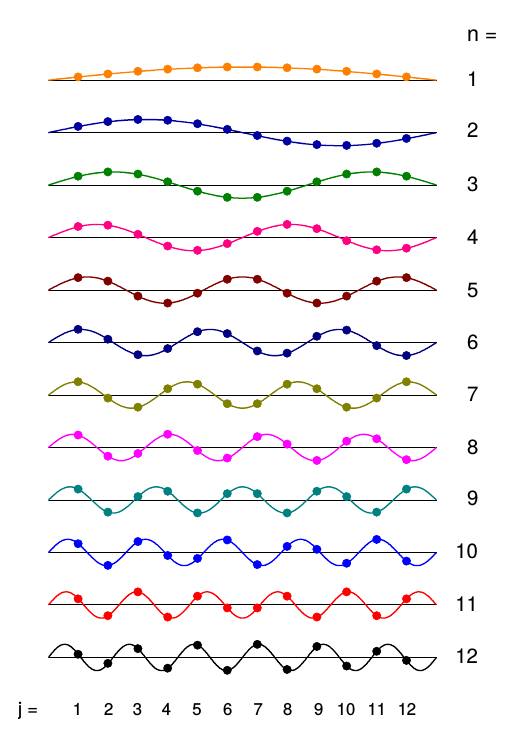
\includegraphics[scale=1.0]{./fig/moden1.png}
  \caption{Schematische Darstellung der $12$ möglichen Schwingungsmoden des Modellkristalls für gleiche Massen \cite{Litmap}}
  \label{fig:moden1}
\end{figure}

\section{Zwei unterschiedliche Massen}

Nun wird auf jeden zweiten Gleiter ein Zusatzgewicht aufgeschraubt. Da eine Basis aus zwei Gleitern besteht, sind nun $6$ unterschiedliche Werte für $k$ möglich. Zu jedem dieser $k$-Werte gehört eine optische und eine akustische Mode, also gibt es insgesamt $12$ Moden (s. Abb. \ref{fig:moden2}).

\begin{figure}[tb]
  \centering
  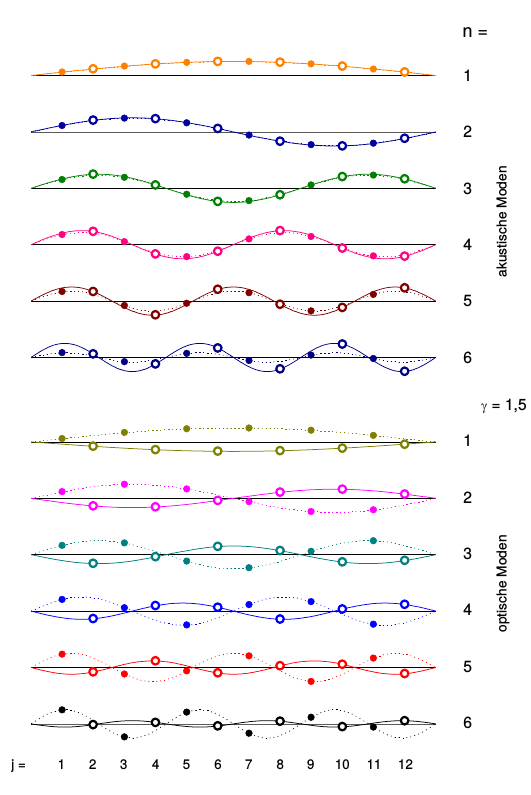
\includegraphics[scale=1.0]{./fig/moden2.png}
  \caption{Schematische Darstellung der $12$ möglichen Schwingungsmoden des Modellkristalls für unterschiedliche Massen \cite{Litmap}}
  \label{fig:moden2}
\end{figure}

Die leichten und die schweren Massen besitzen unterschiedliche maximale Amplituden. Das Verhältnis ist gegeben durch \cite{Litmap}
\begin{equation}
 \frac{s_{0,m}}{s_{0,M}} = \frac{\cos\left(\frac{ka'}{2}\right)}{1-\frac{1+\gamma}{2\gamma}\left(1\pm\sqrt{1-\frac{4\gamma}{(1+\gamma)^{2}}\sin^{2}\left(\frac{ka'}{2}\right)}\right)},
\end{equation}
mit der Gitterkonstante des zweiatomigen Gitters $a'=2a$, der schweren Masse $M$, der leichten Masse $m$ und dem Massenverhältnis $\gamma=\frac{M}{m}$.
Das Amplitudenverhältnis zweier benachbarter Massen ist somit gegeben durch
\begin{equation}
 \frac{s_{0,m}(j)}{s_{0,M}(j-1)} = \frac{s_{0,m}}{s_{0,M}} \frac{\sin\left(\frac{n\pi j}{13}\right)}{\sin\left(\frac{n\pi (j-1)}{13}\right)},
\end{equation}
wenn $j$ der Index der leichten Masse ist und die links benachbarte schwere Masse betrachtet wird.













